\documentclass[aspectratio=169,10pt]{beamer}
\usepackage{amsmath,amssymb}
\usepackage{booktabs}
\usepackage{graphicx}
\usepackage{listings}
\usepackage{xcolor}
\usepackage{hyperref}

% Theme
\usetheme{Madrid}
\usecolortheme{default}

% Title info
\title{Mixture of Experts \& Numerical Precision}
\subtitle{CS290W LLM08 Lecture}
\author{LU Yuzhou}
\date{}

% Code listing style
\definecolor{codebg}{RGB}{245,245,245}
\lstset{
    backgroundcolor=\color{codebg},
    basicstyle=\ttfamily\scriptsize,
    frame=single,
    breaklines=true,
    keywordstyle=\color{blue},
    commentstyle=\color{gray},
    stringstyle=\color{red},
    showstringspaces=false,
    upquote=true,
    literate={__}{{\texttt{\_}\texttt{\_}}}2
             {->}{{$\to$}}2
             {=>}{{$\Rightarrow$}}2,
}

\begin{document}

% Title slide
\frame{\titlepage}

% Slide 1: Overview
\begin{frame}{Lab Overview}
    \textbf{Today's Topics:}
    \begin{enumerate}
        \item \textbf{Mixture of Experts (MoE)}: Sparse activation for efficient scaling
        \item \textbf{Numerical Precision}: FP32, BF16, FP16, FP8 trade-offs
        \item \textbf{Quantization}: INT8/INT4 for model compression
    \end{enumerate}

    \vspace{0.5cm}
    \begin{block}{Why This Matters}
        Modern LLMs (Mixtral, DeepSeek-V3, Qwen3) use MoE to scale to hundreds of billions of parameters while keeping inference practical.
    \end{block}

    \vspace{0.3cm}
    \begin{itemize}
        \item \textbf{Recommended Hardware}: AMD Ryzen AI Halo Processors
        \item \textbf{Environment}: ROCm + PyTorch via AUP Learning Cloud
    \end{itemize}
\end{frame}

% Slide 2: The Scaling Problem
\begin{frame}{The Scaling Dilemma}
    As language models grew, researchers faced a fundamental challenge:

    \vspace{0.5cm}
    \begin{block}{Dense Models Don't Scale Efficiently}
        \begin{itemize}
            \item Larger models $\to$ better quality but proportional compute cost
            \item Training 100B+ dense model: prohibitively expensive
            \item Inference: every token requires ALL parameters
        \end{itemize}
    \end{block}

    \vspace{0.5cm}
    \textbf{Example:} A 100B parameter dense model:
    \begin{itemize}
        \item Memory: 400 GB (FP32)
        \item Compute: 100B ops per token
        \item Inference speed: impractically slow
    \end{itemize}

    \vspace{0.5cm}
    \textbf{Solution:} Decouple \textbf{model capacity} from \textbf{compute cost}
\end{frame}

% Slide 3: MoE Core Idea
\begin{frame}{Mixture of Experts: Core Idea}
    \textbf{Key Insight:} Not all knowledge needs to be activated for every token.

    \vspace{0.3cm}
    \begin{itemize}
        \item Token ``python'' $\to$ activate programming experts
        \item Token ``parrot'' $\to$ activate biology experts
    \end{itemize}

    \vspace{0.3cm}
    \begin{block}{MoE Architecture}
        Instead of one large FFN, use \textbf{multiple smaller FFNs} (``experts'') plus a \textbf{router} that selects which expert(s) to activate.
    \end{block}

    \vspace{0.3cm}
    \textbf{Key Equation:}
    $$y = \sum_{i=1}^{M} G(x)_i \cdot E_i(x)$$
    where $G(x)$ is gating function, $E_i$ is expert $i$.


\end{frame}

% Slide 4: Sparse Activation via Top-K Gating
\begin{frame}{Sparse Activation: Top-K Gating}
    \textbf{Sparsity Mechanism:}
    $$G(x) = \text{softmax}(\text{TopK}(x \cdot W_g))$$

    \vspace{0.3cm}
    \begin{itemize}
        \item Only $k$ experts activated per token (typically $k=1$ or $2$)
        \item \textbf{Model capacity} scales with $M$ (number of experts)
        \item \textbf{Compute cost} stays at $k \times$ single-expert cost
    \end{itemize}

    \vspace{0.3cm}
    \begin{block}{Example: 8 Experts, Top-2}
        \begin{itemize}
            \item Total parameters: 8B (same as dense)
            \item Active parameters: 2B (25\%)
            \item Compute: 4$\times$ less than dense!
        \end{itemize}
    \end{block}

    \vspace{0.3cm}
    \textbf{Router Steps:}
    \begin{enumerate}
        \item Linear projection: $x \cdot W_g$ ($O(d \cdot E)$)
        \item Top-K selection: find $k$ largest ($O(E \log E)$)
        \item Softmax normalization: over $k$ values ($O(k)$)
    \end{enumerate}

    \vspace{0.3cm}
    \begin{center}
        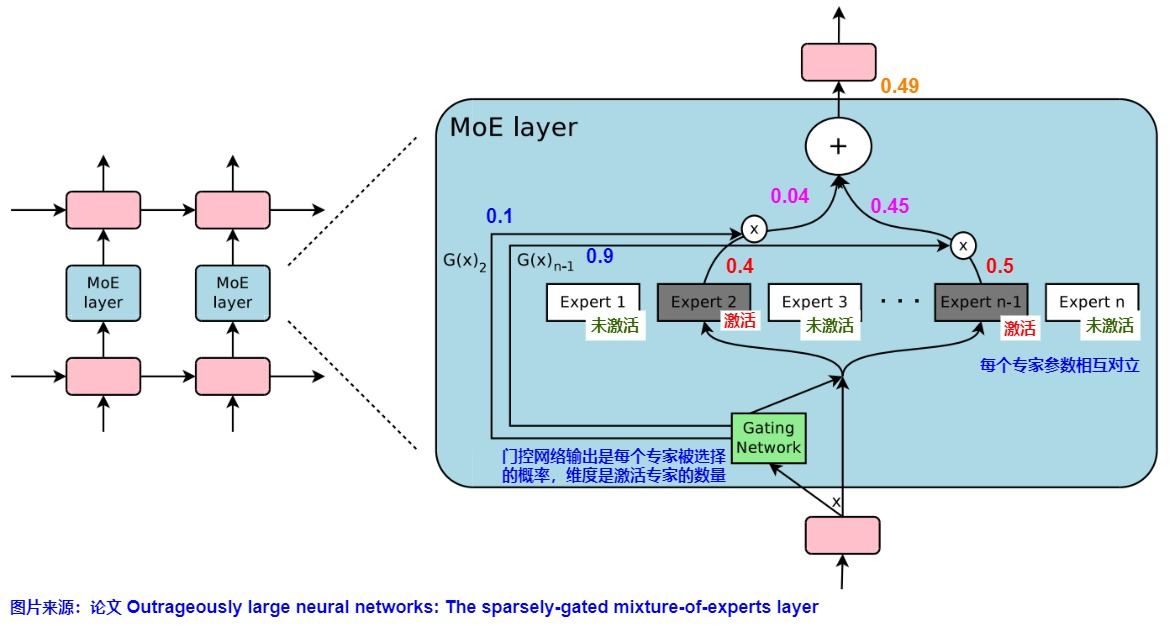
\includegraphics[width=0.55\textwidth]{img/08-gating-network.jpg}
    \end{center}
\end{frame}

% Slide 4b: Gating Network Details
\begin{frame}{Gating Network: Token-to-Expert Routing}
    \begin{center}
        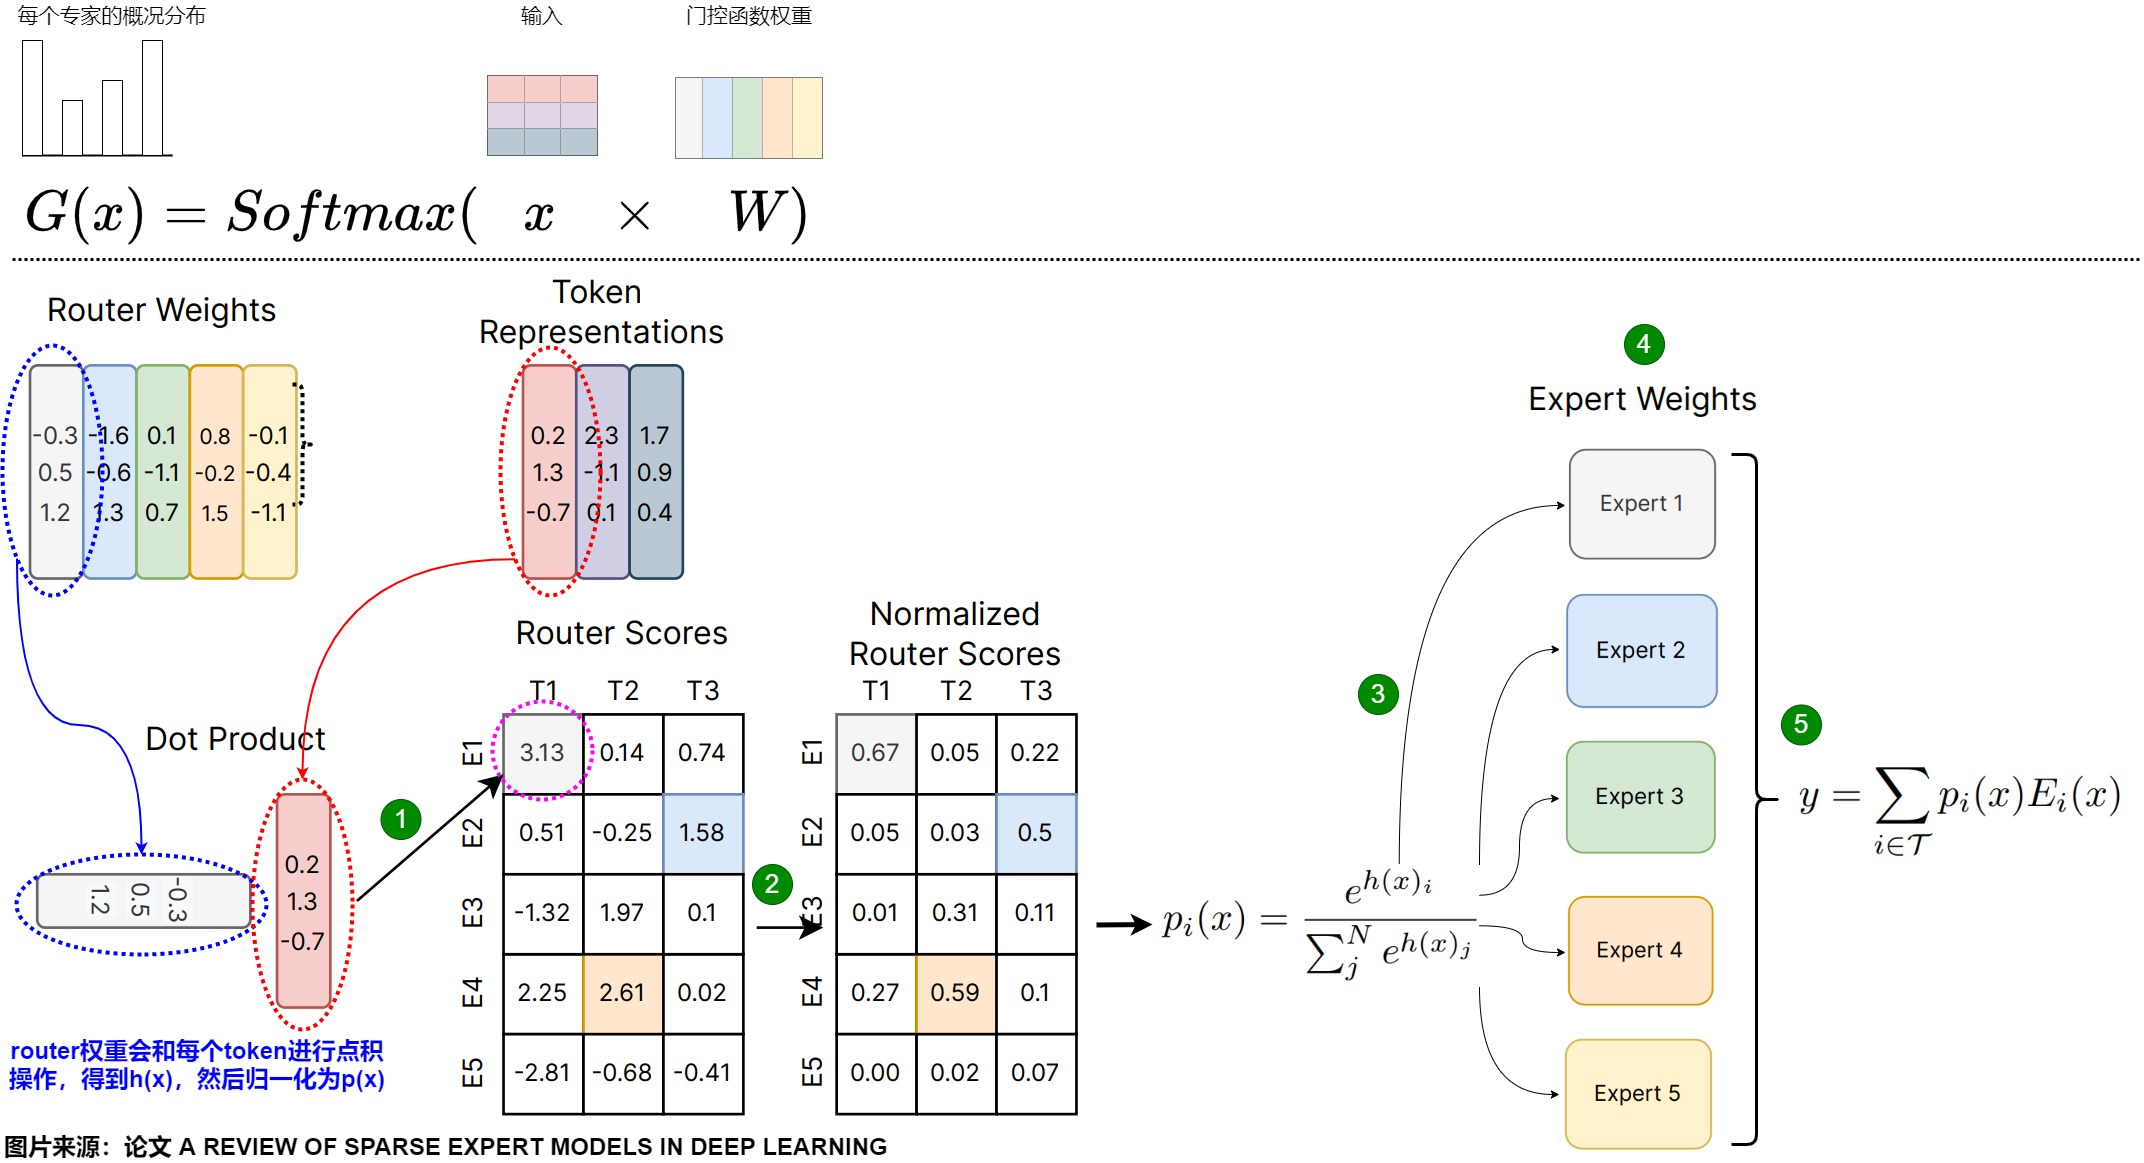
\includegraphics[width=0.85\textwidth]{img/08-moe-routing.jpg}
    \end{center}
\end{frame}
\begin{frame}{Gating Network: Token-to-Expert Routing (Cont'd)}
    \vspace{0.3cm}
    \textbf{Routing Process:}
    \begin{enumerate}
        \item Input tokens (colored) are processed by router
        \item Router computes weights ($W$) for each expert
        \item Dot product produces routing scores $h(x)$
        \item Softmax normalizes to probabilities $p(x)$
        \item Top-K experts selected per token
    \end{enumerate}

    \vspace{0.3cm}
    \begin{block}{Key Point}
        Each expert receives only the tokens it's specialized to process, enabling efficient computation.
    \end{block}
\end{frame}

% Slide 5: MoE vs Dense Comparison
\begin{frame}{MoE vs Dense: 8B Model Comparison}
    \begin{table}
        \centering
        \small
        \begin{tabular}{lrr}
            \toprule
            \textbf{Metric} & \textbf{Dense 8B} & \textbf{MoE 8B (8 experts, top-2)} \\
            \midrule
            Total Parameters & 8B & 8B \\
            Active Parameters & 8B (100\%) & 2B (25\%) \\
            Memory Footprint & 32 GB (FP32) & 32 GB (FP32) \\
            Compute per Token & 8B ops & ~2B ops (4$\times$ less) \\
            Inference Speed & 1$\times$ & ~3-4$\times$ faster* \\
            \bottomrule
        \end{tabular}
    \end{table}

    \vspace{0.5cm}
    \begin{block}{Key Advantage}
        MoE achieves GPT-level quality with \textbf{manageable inference cost} by activating only a subset of parameters.
    \end{block}

    \vspace{0.3cm}
    {\footnotesize *Speedup depends on implementation efficiency and memory bandwidth}
\end{frame}

% Slide 6: Transformer Layer Structure
\begin{frame}{Where Does MoE Fit in Transformer?}
    Standard Transformer layer:

    \vspace{0.3cm}
    \begin{center}
    \begin{tabular}{l}
        Input \\
        $\downarrow$ \\
        \fbox{Multi-Head Attention (MHA)} \textcolor{red}{← CANNOT be MoE} \\
        $\downarrow$ \\
        \fbox{Feed-Forward Network (FFN)} \textcolor{green}{← CAN be replaced with MoE} \\
        $\downarrow$ \\
        Output
    \end{tabular}
    \end{center}

    \vspace{0.5cm}
    \textbf{Why MHA Cannot Be MoE:}
    \begin{itemize}
        \item \textbf{Token Mixing:} Each query must attend to ALL keys
        \item \textbf{Context Dependency:} Output for token $i$ depends on all tokens $j$
        \item \textbf{Mathematical Structure:} $QK^T$ creates $N \times N$ attention matrix
        \item Sparse activation would break global context flow
    \end{itemize}


\end{frame}

% Slide 7: LLaMA-Style FFN Expert
\begin{frame}{LLaMA-Style FFN Expert: SwiGLU}
    Each expert uses the \textbf{SwiGLU} (Swish Gated Linear Unit) activation:

    \vspace{0.2cm}
    \begin{block}{Standard FFN (pre-LLaMA)}
        $$\text{FFN}(x) = W_2 \cdot \text{ReLU}(W_1 \cdot x)$$
    \end{block}

    \vspace{0.2cm}
    \begin{block}{LLaMA FFN with SwiGLU}
        $$\text{FFN}(x) = W_{\text{down}} \cdot \Big(\text{SiLU}(W_{\text{gate}} \cdot x) \otimes (W_{\text{up}} \cdot x)\Big)$$
        where $\otimes$ is element-wise multiplication.
    \end{block}

    \vspace{0.2cm}
    \begin{table}
        \centering
        \small
        \begin{tabular}{lll}
            \toprule
            \textbf{Layer} & \textbf{Shape} & \textbf{Purpose} \\
            \midrule
            gate\_proj & $d \to d_{\text{inter}}$ & Produces gate activations \\
            up\_proj & $d \to d_{\text{inter}}$ & Produces value activations \\
            down\_proj & $d_{\text{inter}} \to d$ & Projects back to hidden dim \\
            SiLU & -- & $\text{SiLU}(x) = x \cdot \sigma(x)$ \\
            \bottomrule
        \end{tabular}
    \end{table}

    \vspace{0.3cm}
    \textbf{Compute Cost:} $O(3 \cdot d \cdot d_{\text{inter}})$ per token
\end{frame}

% Slide 8: Router Compute Cost Analysis
\begin{frame}{Router Compute: Is It Expensive?}
    Router computes: $G(x) = \text{softmax}(\text{TopK}(x \cdot W_g))$

    \vspace{0.2cm}
    \textbf{Compute Breakdown per Token:}
    \begin{enumerate}
        \item Linear projection $x \cdot W_g$: $O(d \cdot E)$
        \item Top-K selection: $O(E \log E)$
        \item Softmax over $k$ values: $O(k)$
    \end{enumerate}

    \vspace{0.2cm}
    \begin{block}{Example: $d=4096$, $E=8$, $k=2$}
        \begin{itemize}
            \item Router: ~32K ops/token
            \item Expert FFN: ~131M ops/token
            \item \textbf{Router overhead: ~0.02\%} (negligible!)
        \end{itemize}
    \end{block}

    \vspace{0.2cm}
    \begin{block}{Combine Layer Cost}
        Combining expert outputs: $O(k \cdot d)$ per token \\
        For $k=2$, $d=4096$: negligible compared to expert compute.
    \end{block}
\end{frame}

% Slide 9: MoE Penalties
\begin{frame}{MoE Penalties vs Dense Models}
    Despite compute savings, MoE introduces challenges:

    \vspace{0.5cm}
    \begin{table}
        \centering
        \small
        \begin{tabular}{lll}
            \toprule
            \textbf{Penalty} & \textbf{Description} & \textbf{Impact} \\
            \midrule
            Communication & All-to-all in distributed training & 10-30\% slowdown \\
            Load Imbalance & Uneven expert utilization & Wasted compute \\
            Router Compute & Gating network overhead & ~5\% (small) \\
            \bottomrule
        \end{tabular}
    \end{table}

    \vspace{0.5cm}
    \textbf{Load Imbalance Problem:}
    \begin{itemize}
        \item Without constraints, router tends to favor few ``popular'' experts
        \item Some experts over-trained, others under-trained
        \item GPU load imbalance in distributed training/inferring
    \end{itemize}

    \vspace{0.5cm}
    \textbf{Solution:} Add \textbf{load-balancing auxiliary loss}
\end{frame}

% Slide 10: Load Balancing Loss
\begin{frame}{Load Balancing Loss}
    \textbf{Switch Transformer Auxiliary Loss:}
    $$\mathcal{L}_{\text{balance}} = \alpha \cdot N_E \cdot \sum_{i=1}^{N_E} f_i \cdot P_i$$

    \vspace{0.2cm}
    Where:
    \begin{itemize}
        \item $f_i$ = fraction of tokens routed to expert $i$
        \item $P_i$ = average router probability for expert $i$
        \item $N_E$ = number of experts
    \end{itemize}

    \vspace{0.2cm}
    \begin{block}{How It Works}
        The loss penalizes:
        \begin{itemize}
            \item Experts that receive too many tokens (high $f_i$)
            \item Experts with high average probabilities (high $P_i$)
        \end{itemize}
        Result: encourages \textbf{uniform expert utilization}.
    \end{block}

    \vspace{0.1cm}
    {\footnotesize \textit{Note: DeepSeek-V3 uses shared experts with capacity constraints instead.}}
\end{frame}

% Slide 10b: Gating Functions Comparison
\begin{frame}{Gating Functions: Different Routing Strategies}
    \begin{center}
        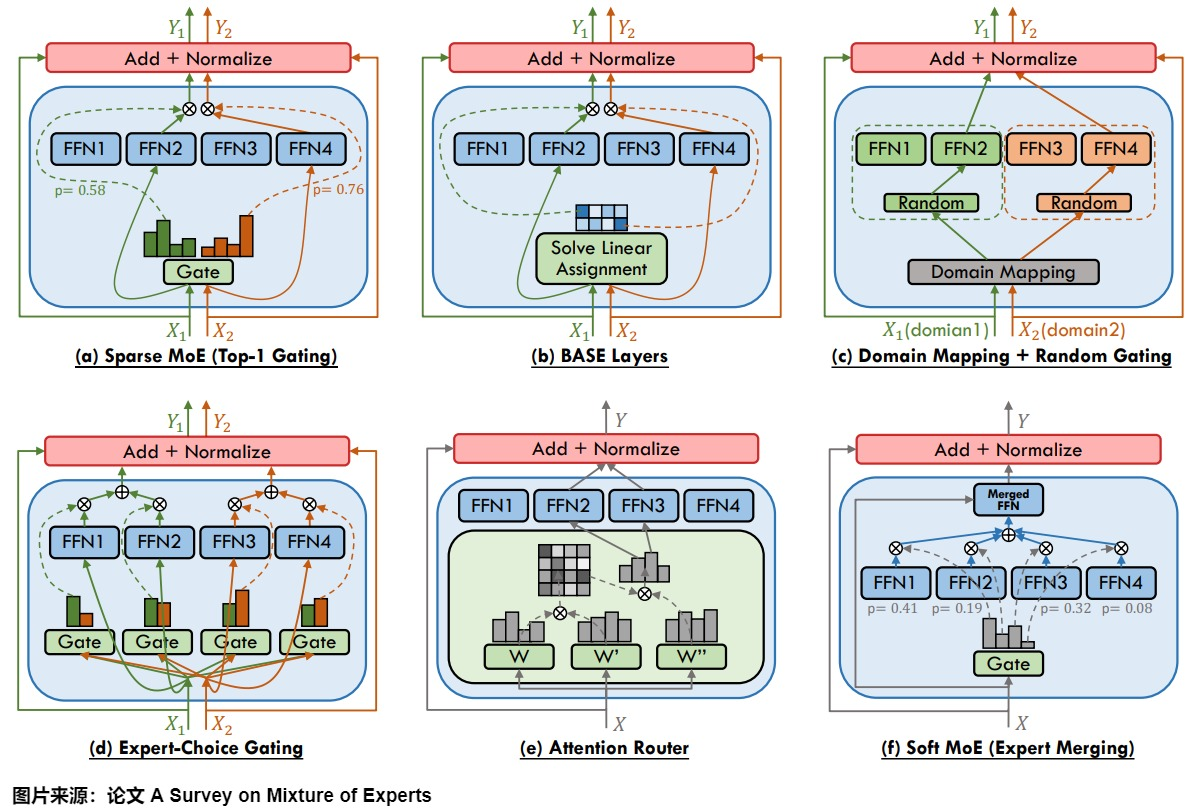
\includegraphics[width=0.75\textwidth]{img/08-gating-functions.jpg}
    \end{center}
\end{frame}
\begin{frame}{Gating Functions: Different Routing Strategies(Cont.)}
    \vspace{0.3cm}
    \textbf{Common Gating Strategies:}
    \begin{itemize}
        \item \textbf{(a) Top-1 gating:} Select single best expert (Switch Transformer)
        \item \textbf{(b) BASE layer:} Balanced assignment with soft weighting
        \item \textbf{(c) Stochastic gating:} Random selection with domain mapping
        \item \textbf{(d) Expert selection:} Multiple experts per token
        \item \textbf{(e) Attention router:} Attention-based routing scores
        \item \textbf{(f) Soft MoE:} All experts with learned merging
    \end{itemize}
\end{frame}

% Slide 11: Notable MoE Models
\begin{frame}{Notable MoE Models in Production}
    \begin{table}
        \centering
        \small
        \begin{tabular}{lrrl}
            \toprule
            \textbf{Model} & \textbf{\#Experts} & \textbf{Top-K} & \textbf{Notes} \\
            \midrule
            Mixtral 8$\times$7B & 8 & 2 & Popular open-source MoE \\
            Mixtral 8$\times$22B & 8 & 2 & Larger experts \\
            DeepSeek-V3 & 256+1 & 8+1 & Shared expert + routing \\
            Qwen3-235B-A22B & 128 & 8 & Alibaba open-source \\
            \bottomrule
        \end{tabular}
    \end{table}

    \vspace{0.5cm}
    \begin{block}{DeepSeek-V3 Configuration}
        \begin{itemize}
            \item Total: 670B parameters, 37B active
            \item 256 routed experts + 1 shared expert
            \item Top-8 from routed + always use shared
            \item Achieves GPT-4 level quality with efficient inference
        \end{itemize}
    \end{block}

    \vspace{0.3cm}

\end{frame}

% Slide 12: Floating-Point Formats
\begin{frame}{Floating-Point Format Comparison}
    \begin{table}
        \centering
        \small
        \begin{tabular}{lrrrrl}
            \toprule
            \textbf{Format} & \textbf{Sign} & \textbf{Exp} & \textbf{Mantissa} & \textbf{Range} & \textbf{Use Case} \\
            \midrule
            FP32 & 1 & 8 & 23 & $\pm 3.4 \times 10^{38}$ & Full-precision training \\
            BF16 & 1 & 8 & 7 & $\pm 3.4 \times 10^{38}$ & Large-scale training \\
            FP16 & 1 & 5 & 10 & $\pm 6.55 \times 10^{4}$ & Mixed-precision \\
            FP8 E4M3 & 1 & 4 & 3 & $\pm 448$ & Latest GPU inference \\
            FP8 E5M2 & 1 & 5 & 2 & $\pm 5.7 \times 10^{4}$ & Latest GPU training \\
            \bottomrule
        \end{tabular}
    \end{table}

    \vspace{0.5cm}
    \begin{block}{Trade-offs}
        \begin{itemize}
            \item \textbf{More exponent bits} $\to$ wider dynamic range
            \item \textbf{More mantissa bits} $\to$ higher precision
            \item BF16: same range as FP32, less precision (good for training)
            \item FP16: higher precision but narrow range (overflow risk)
        \end{itemize}
    \end{block}
\end{frame}

% Slide 13: Mixed Precision Training
\begin{frame}{Mixed Precision Training}
    \textbf{Idea:} Combine FP32 (master weights) with FP16/BF16 (compute)


    \begin{block}{Benefits}
        \begin{itemize}
            \item \textbf{Halve} memory usage
            \item \textbf{Double} throughput on Tensor Cores
            \item Maintain FP32-level training accuracy
        \end{itemize}
    \end{block}

    \textbf{Typical Flow:}
    \begin{enumerate}
        \item Forward pass in FP16/BF16
        \item Loss computed in FP32 (with loss scaling for FP16)
        \item Backward pass in FP16/BF16
        \item Weight update in FP32 (master copy)
    \end{enumerate}

    \begin{block}{Memory Savings}
        For a 1B parameter model:
        \begin{itemize}
            \item FP32: 4 GB
            \item FP16/BF16: 2 GB (\textbf{50\% savings})
        \end{itemize}
    \end{block}
\end{frame}

% Slide 14: Quantization Basics
\begin{frame}{Quantization: Model Compression}
    \textbf{Goal:} Map floating-point weights to lower-bit integers.


    \begin{block}{Symmetric Quantization Formulas}
        \begin{align*}
            \text{scale} &= \frac{\max(|x|)}{q_{\max}} \\
            x_q &= \text{round}\left(\frac{x}{\text{scale}}\right), \text{clipped to } [q_{\min}, q_{\max}] \\
            x_{\text{dequantized}} &= x_q \cdot \text{scale}
        \end{align*}
    \end{block}


    Where:
    \begin{itemize}
        \item $q_{\min} = -(2^{\text{bits}-1})$ (e.g., -128 for INT8)
        \item $q_{\max} = 2^{\text{bits}-1} - 1$ (e.g., 127 for INT8)
    \end{itemize}


    \begin{block}{Quantization Approaches}
        \begin{itemize}
            \item \textbf{Post-Training Quantization (PTQ):} Quantize after training
            \item \textbf{Quantization-Aware Training (QAT):} Train with fake-quantize
            \item \textbf{Weight-only INT8/INT4:} Quantize weights, keep activations FP16
        \end{itemize}
    \end{block}
\end{frame}

% Slide 15: Quantization Impact
\begin{frame}{Quantization: Size vs Accuracy Trade-off}
    \begin{table}
        \centering
        \small
        \begin{tabular}{lrrr}
            \toprule
            \textbf{Format} & \textbf{Bits} & \textbf{Size Reduction} & \textbf{Typical Error} \\
            \midrule
            FP32 & 32 & 1$\times$ & 0.000000 \\
            INT8 & 8 & 4$\times$ & ~0.001-0.01 \\
            INT4 & 4 & 8$\times$ & ~0.01-0.1 \\
            \bottomrule
        \end{tabular}
    \end{table}

    \vspace{0.5cm}
    \begin{block}{Example: 1B Parameter Model}
        \begin{itemize}
            \item FP32: 4 GB
            \item INT8: 1 GB (\textbf{4$\times$ smaller})
            \item INT4: 0.5 GB (\textbf{8$\times$ smaller})
        \end{itemize}
    \end{block}

    \vspace{0.5cm}
    \textbf{Use Cases:}
    \begin{itemize}
        \item INT8: Production inference (minimal accuracy loss)
        \item INT4: Edge deployment, mobile (acceptable accuracy loss)
    \end{itemize}
\end{frame}

% Slide 16: Lab Implementation Overview
\begin{frame}[fragile]{Lab: What You'll Implement}
    \textbf{Step 1: Top-K Gating Network}
    \begin{lstlisting}[language=Python]
class TopKGating(nn.Module):
    def forward(self, x):
        scores = self.router(x)           # (B, S, E)
        topk_scores, topk_idx = torch.topk(scores, k)
        probs = torch.softmax(topk_scores, dim=-1)
        gate = torch.zeros_like(scores)
        gate.scatter_(-1, topk_idx, probs)  # sparse gate
        return gate, topk_idx
    \end{lstlisting}

    \vspace{0.1cm}
    \textbf{Step 2: LLaMA-Style Expert}
    \begin{lstlisting}[language=Python]
class Expert(nn.Module):
    def forward(self, x):
        return self.down_proj(
            self.act_fn(self.gate_proj(x)) * self.up_proj(x)
        )
    \end{lstlisting}

    \vspace{0.1cm}
    \textbf{Step 3: Assemble MoE Layer}
    \begin{itemize}
        \item Route tokens to experts
        \item Combine weighted outputs
        \item Compute load balancing loss
    \end{itemize}
\end{frame}

% Slide 17: Lab: Quantization Exercise
\begin{frame}[fragile]{Lab: Quantization Exercise}
    \textbf{Implement Symmetric Quantization:}
    \begin{lstlisting}[language=Python]
def quantize_tensor(x, num_bits=8):
    qmin = -(2 ** (num_bits - 1))
    qmax = 2 ** (num_bits - 1) - 1
    scale = x.abs().max() / qmax
    x_q = torch.clamp(torch.round(x / scale), qmin, qmax)
    return x_q, scale

def dequantize_tensor(x_q, scale):
    return x_q.float() * scale
    \end{lstlisting}


    \textbf{Experiments:}
    \begin{itemize}
        \item Quantize MLP weights to INT8 and INT4
        \item Measure reconstruction error
        \item Compare FP32 vs quantized model output
    \end{itemize}


    \begin{block}{Expected Results}
        INT8: mean abs error ~0.001 \\
        INT4: mean abs error ~0.01 (higher, but 8$\times$ compression)
    \end{block}
\end{frame}

% Slide 18: Summary
\begin{frame}{Summary: Key Takeaways}
    \begin{enumerate}
        \item \textbf{MoE Architecture}: Sparse activation via Top-K gating
        \begin{itemize}
            \item Scales capacity without scaling compute
            \item Only FFN layer can be MoE (not attention)
        \end{itemize}

        \item \textbf{Router}: Linear + TopK + Softmax + scatter
        \begin{itemize}
            \item Negligible overhead (~0.02\%)
            \item Creates sparse gate with $k$ nonzero values
        \end{itemize}

        \item \textbf{Load Balancing}: Auxiliary loss prevents expert collapse

        \item \textbf{Floating-Point}: BF16 (wide range), FP16 (higher precision)

        \item \textbf{Quantization}: INT8/INT4 for inference compression
        \begin{itemize}
            \item Symmetric quantization: $x_q = \text{round}(x / \text{scale})$
            \item Trade-off: size vs accuracy
        \end{itemize}
    \end{enumerate}
\end{frame}

% Slide 19: Experiment Further
\begin{frame}{Experiment Further}
    \begin{itemize}
        \item Modify \texttt{top\_k} from 2 to 1: observe expert distribution change
        \item Compare per-channel vs per-tensor quantization accuracy
        \item Apply quantization to real LLaMA model using \texttt{bitsandbytes}
        \item Implement capacity factor to limit max tokens per expert
        \item Benchmark MoE vs dense FFN with same compute budget
    \end{itemize}

    \vspace{0.5cm}
    \begin{block}{Resources}
        \begin{itemize}
            \item \textbf{Mixtral Paper}: \href{https://arxiv.org/abs/2401.04088}{arXiv:2401.04088}
            \item \textbf{Switch Transformer}: \href{https://arxiv.org/abs/2101.03961}{arXiv:2101.03961}
            \item \textbf{DeepSeek-V3}: \href{https://arxiv.org/abs/2412.19437}{arXiv:2412.19437}
            \item \textbf{Lab Notebook}: \texttt{LLM08-MoE-and-Numerical-Precision.ipynb}
        \end{itemize}
    \end{block}
\end{frame}



\end{document}
